\chapter{Testing}
\section{Test Plan}
To test software, a plan must be set out to efficiently capture all bugs and to test the accuracy and precision of the said software. The goal of this section is to devise an efficient testing plan. \\
My project is not very edge-case intensive, each component in my project works with one another and if one breaks, then the whole project stops making sense. Since this is the case, catching a bug is critical, however, bugs are rare since they are so easy to catch. My plan is to pick different tests, and to apply those tests in different locations of the globe, multiple times. That way, I can efficiently find any bugs, glitches or unexpected behaviour. I will also be testing the \textit{accuracy} of my project, by comparing values with real, trusted data banks.
\newpage
\section{Accuracy Testing}
\begin{enumerate}
    \item Objective: Select 'United States' \\
        Test Result: \textbf{Passed}
\begin{figure}[h]
\centering
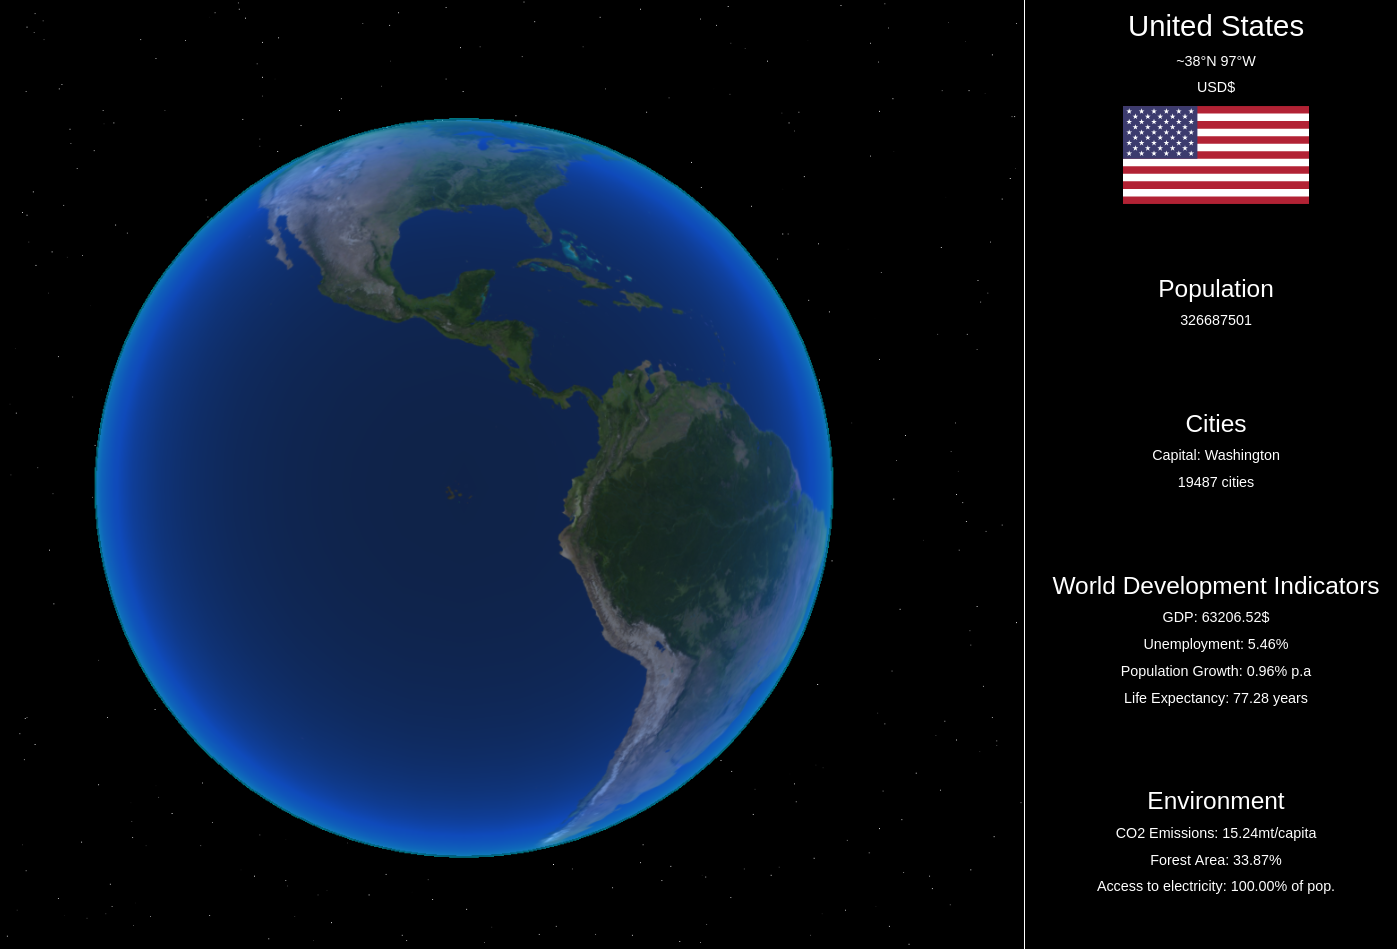
\includegraphics[width=0.4\linewidth]{images/usa}
\end{figure}
    \item Objective: Select 'Spain' \\
        Test Result: \textbf{Passed}
\begin{figure}[ht]
\centering
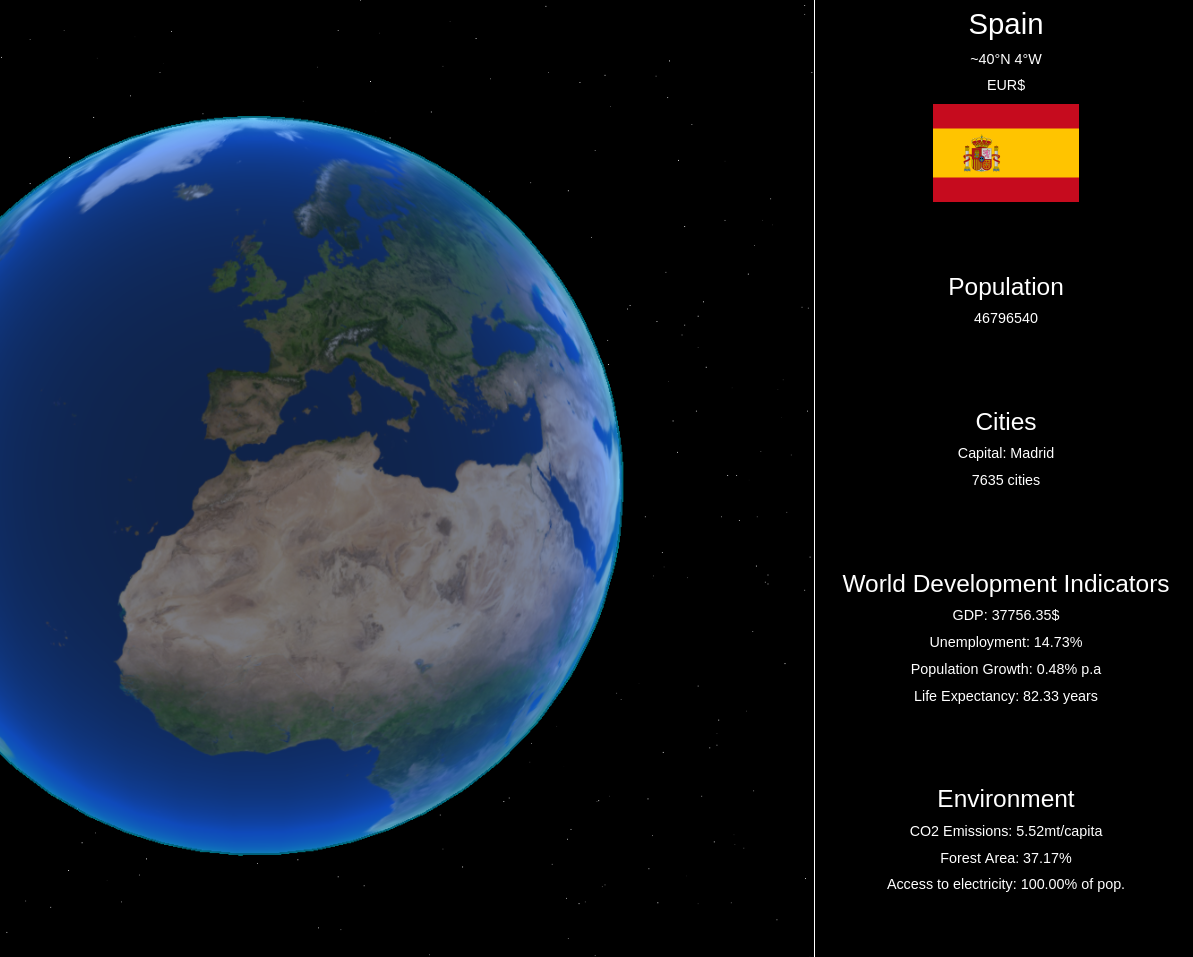
\includegraphics[width=0.4\linewidth]{images/spain}
\end{figure}
    \item Objective: Select 'Portugal' \\
        Test Result: \textbf{Passed}
\begin{figure}[ht]
\centering
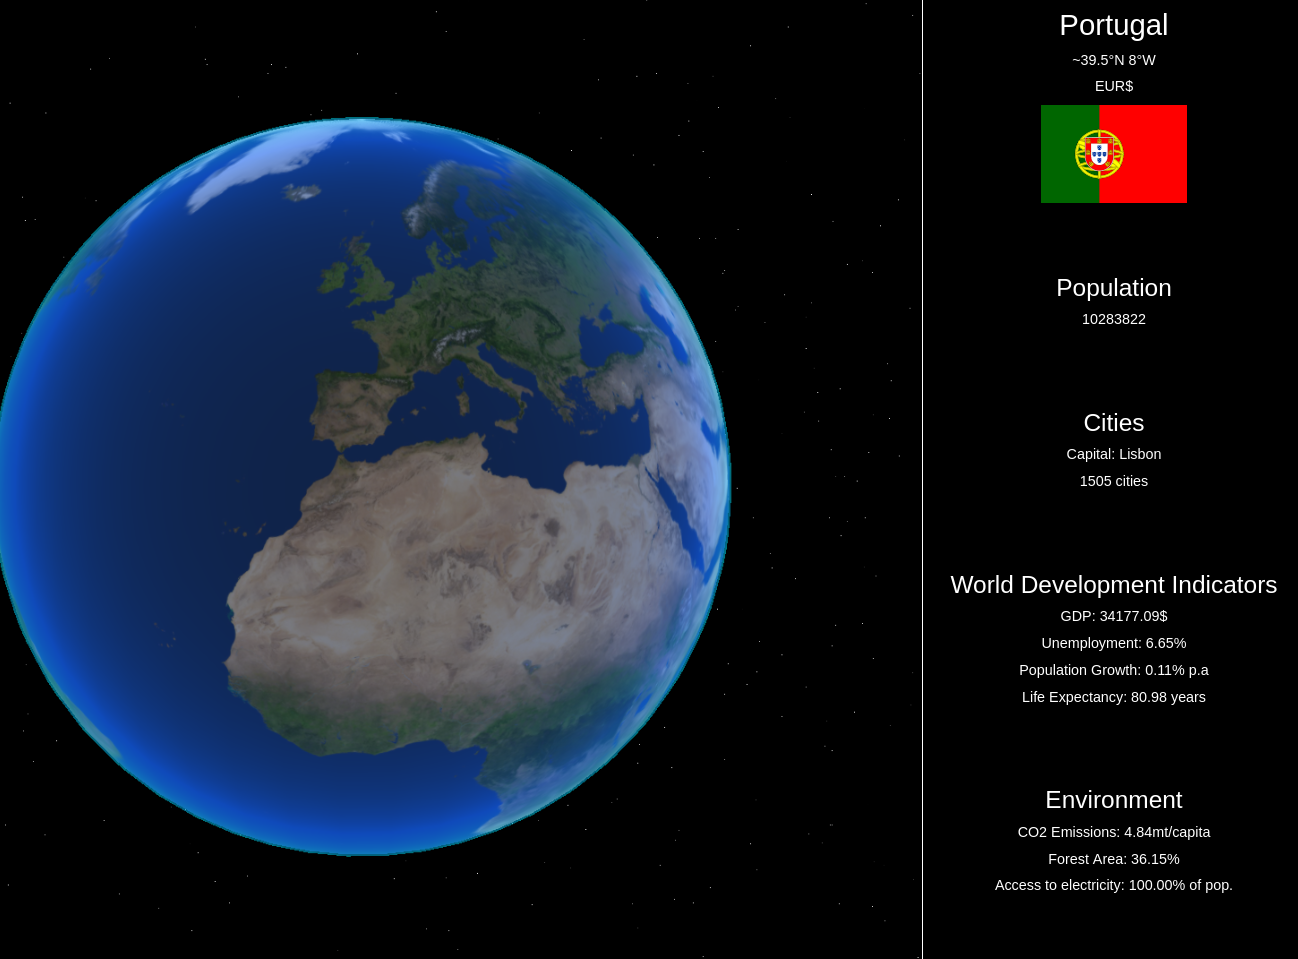
\includegraphics[width=0.4\linewidth]{images/pt}
\end{figure}
\newpage
    \item Objective: Select 'Luxembourg' \\
        Test Result: \textbf{Passed} \\
        Note: Needed to zoom in to accurately select it.
\begin{figure}[ht]
\centering
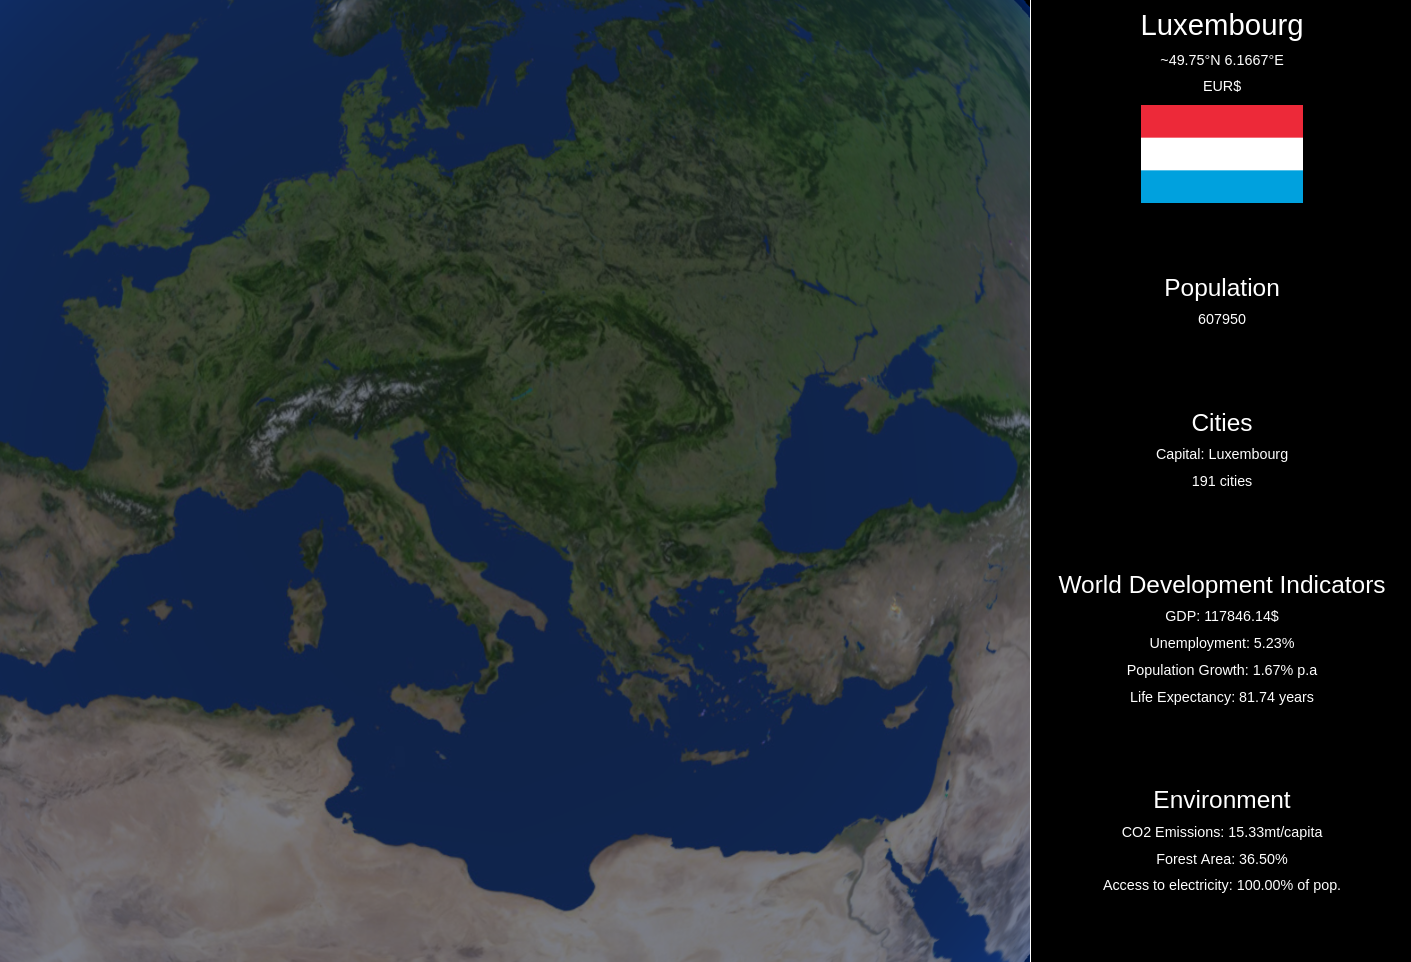
\includegraphics[width=0.4\linewidth]{images/luxembourg}
\end{figure}
    \item Objective: Select 'Italy' \\
        Test Result: \textbf{Failed} \\
        Note: Kept selecting San Marino \& Vatican City due to their extreme proximity to italy.
\begin{figure}[ht]
\centering
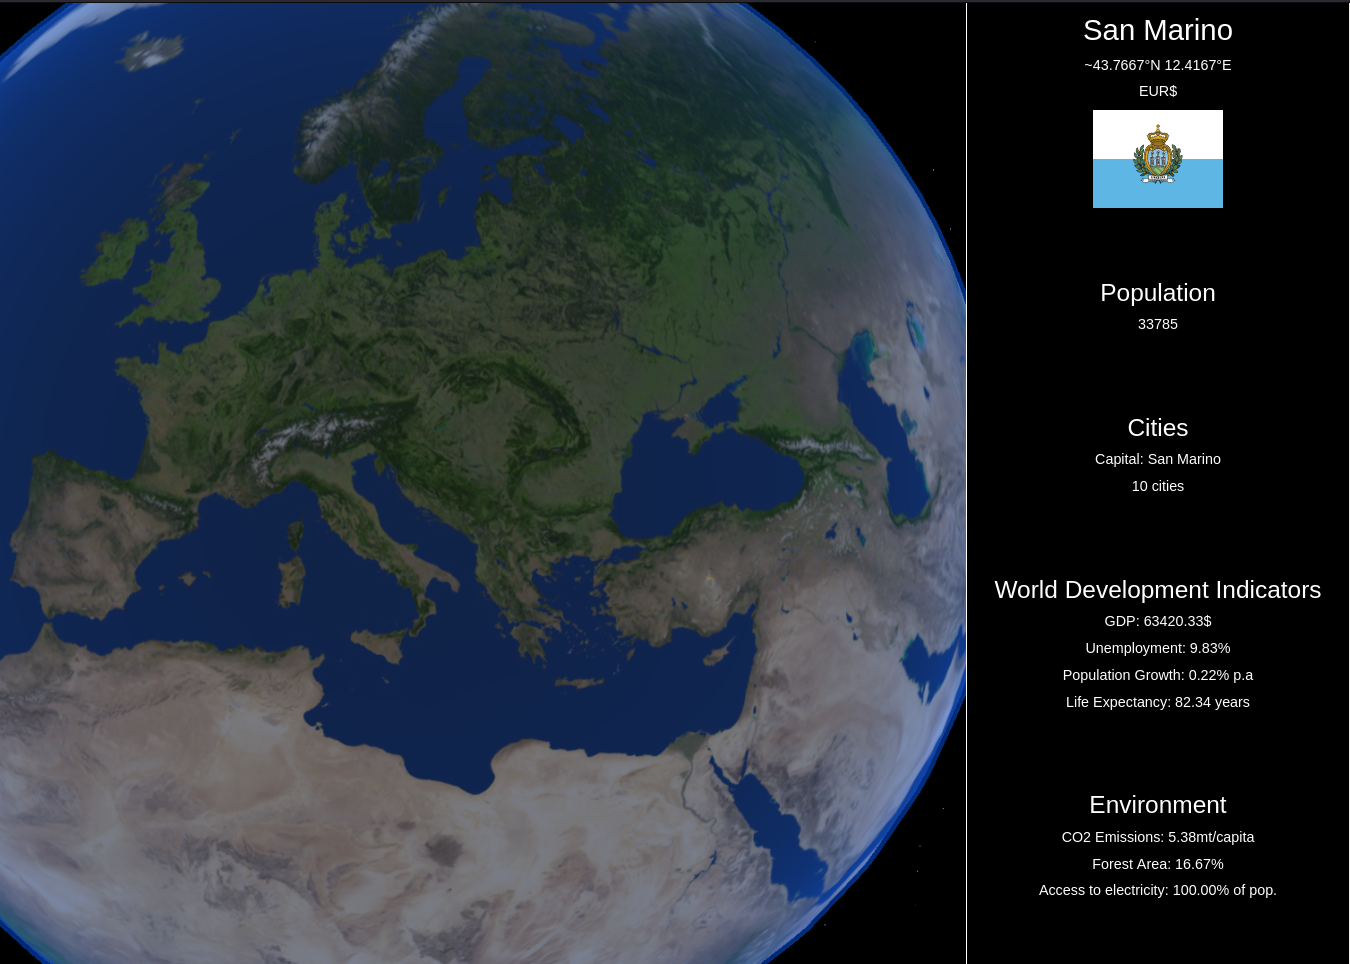
\includegraphics[width=0.4\linewidth]{images/italy}
\end{figure}
    \item Objective: Select 'Cape Verde' \\
        Test Result: \textbf{Passed} \\
\begin{figure}[ht]
\centering
\newpage
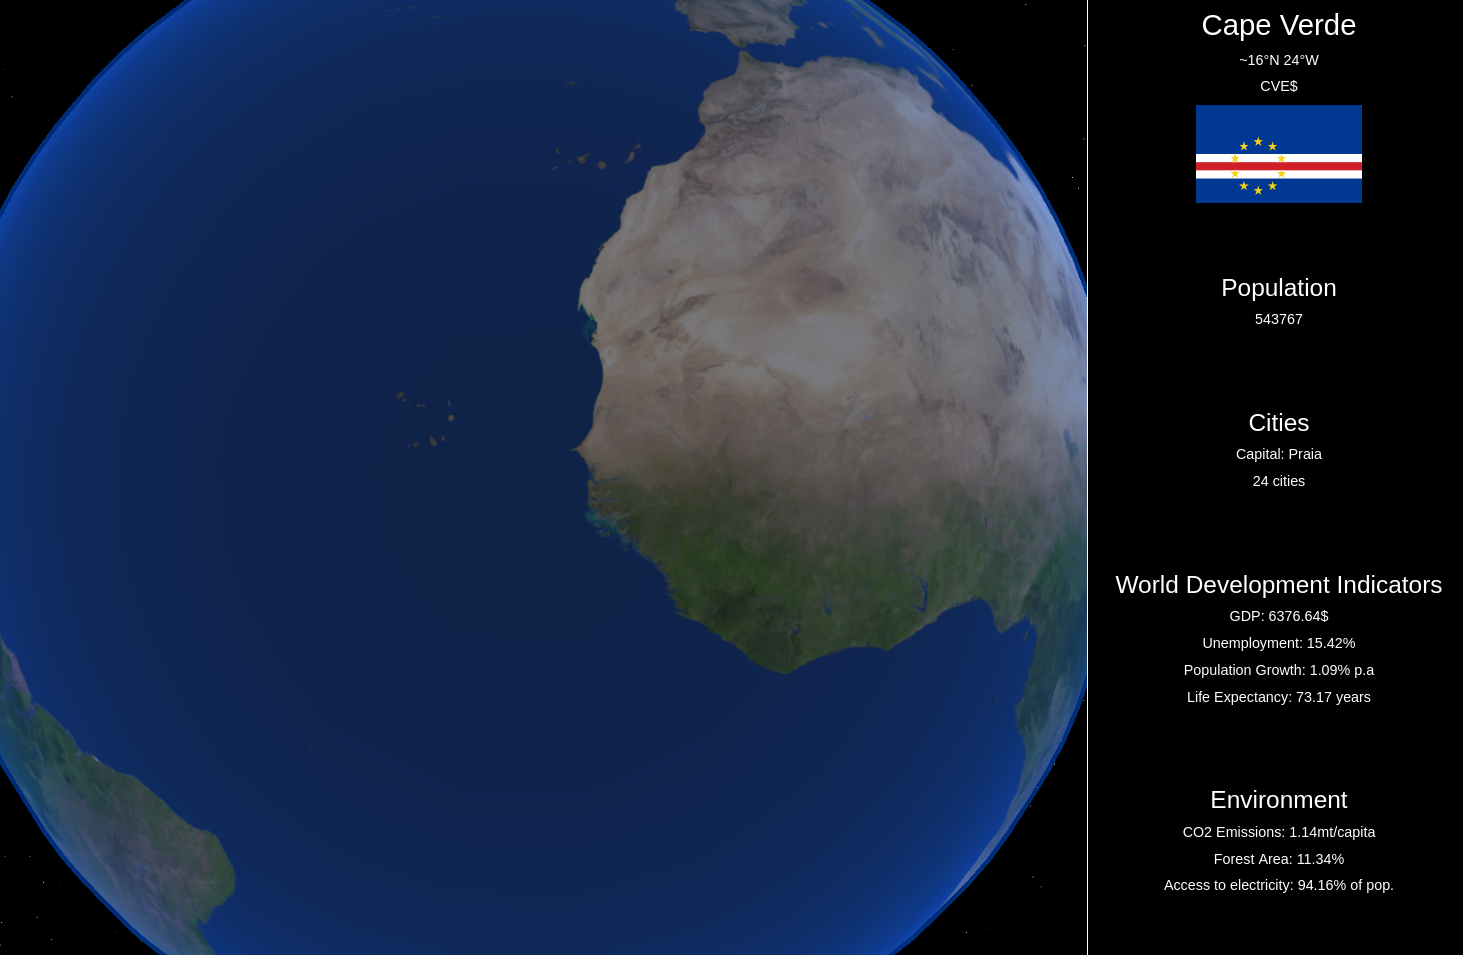
\includegraphics[width=0.4\linewidth]{images/capeverde}
\end{figure}
    \item Objective: Select 'Falkland Islands' \\
        Test Result: \textbf{Passed} \\
        Note: Inconclusive world bank indicator API results.
\begin{figure}[ht]
\centering
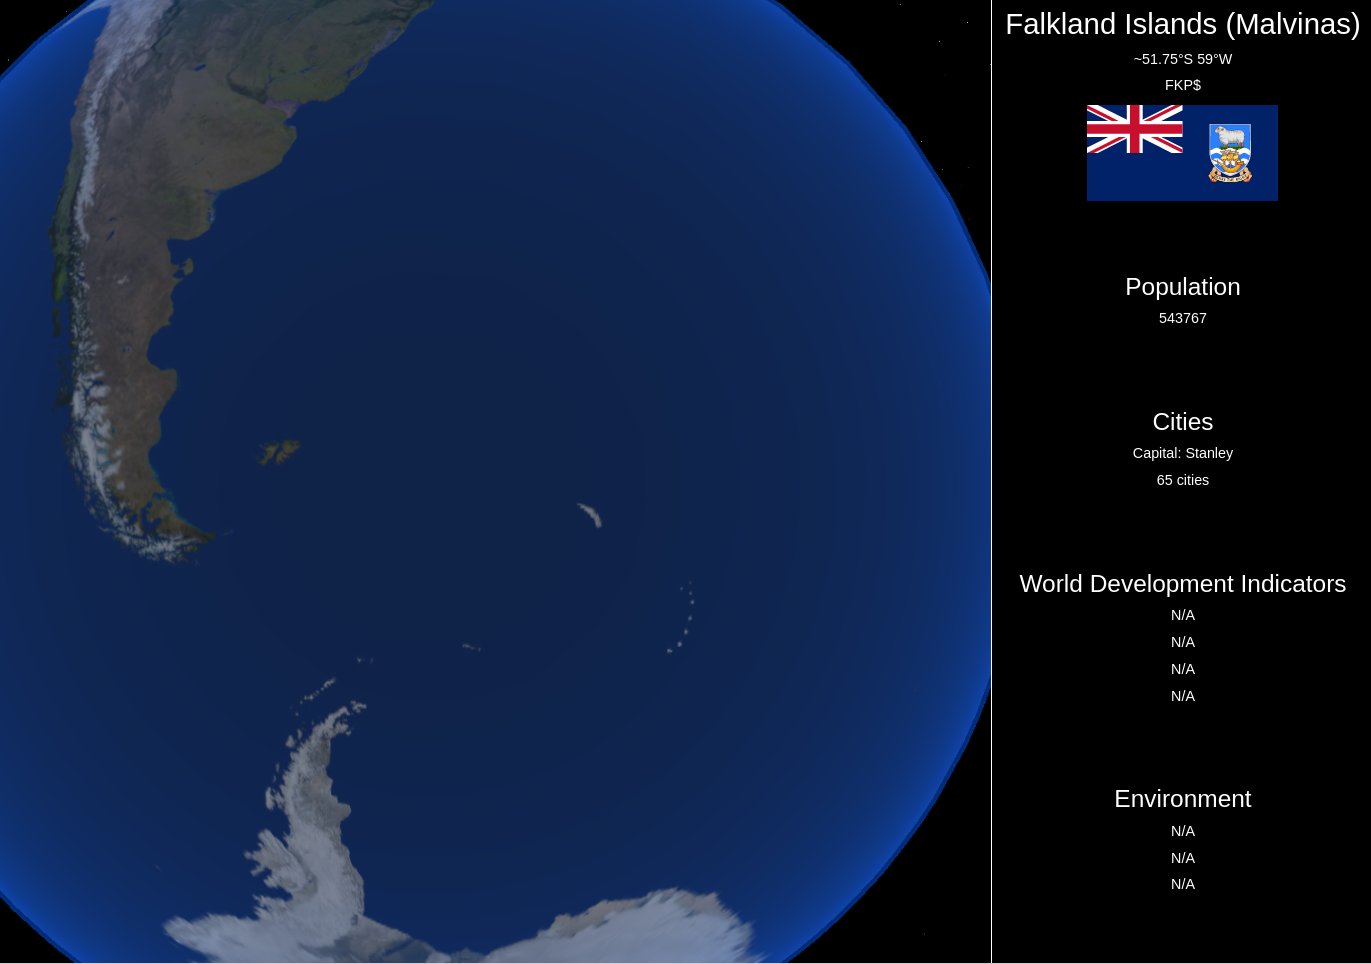
\includegraphics[width=0.4\linewidth]{images/falklands}
\end{figure}
\end{enumerate}

\subsection{Test Conclusion}
In conclusion, I think that the tests were quite successful. It can select even small islands, and most of europe passes the test. However, countries like Italy failed due to it's enclaves (Vatican City, San Marino microstate). This could be solved by using a different model for country selection such as the complex country border mapping model, which involves mapping borders onto the globe, and calculating selection that way. I'd say that my model is actually quite accurate, and for most cases, it can get the country right the very first attempt.

\newpage
\section{API Testing}
I will only be testing the population variable and the GDP variable to save time. Population \& GDP is compared with CIA estimate.\footnote{https://www.cia.gov/the-world-factbook/field/real-gdp-per-capita/country-comparison}
\begin{enumerate}
    \item Objective: Test 'Portugal' \\
        Comparison:
        \begin{itemize}
            \item \textbf{GDP per capita (PPP)} \\
                Result: 34,177\$ \\
                Real: 32,000\$
            \item \textbf{Population} \\
                Result: 10,283,822 \\
                Real: 10,142,236
        \end{itemize}
    \item Objective: Test 'Iceland' \\
        Comparison:
        \begin{itemize}
            \item \textbf{GDP per capita (PPP)} \\
                Result: 53,616\$ \\
                Real: 52,300\$
            \item \textbf{Population} \\
                Result: 352,721 \\
                Real: 357,603 \\
        \end{itemize}
    \item Objective: Test 'Madagascar' \\
        Comparison:
        \begin{itemize}
            \item \textbf{GDP per capita (PPP)} \\
                Result: 1,544\$ \\
                Real: 1,500\$
            \item \textbf{Population} \\
                Result: 26,262,368 \\
                Real: 28,172,462 \\
        \end{itemize}
\newpage
    \item Objective: Test 'Falkland Islands' \\
        Comparison:
        \begin{itemize}
            \item \textbf{GDP per capita (PPP)} \\
                Result: N/A\$ \\
                Real: 70,800\$
            \item \textbf{Population} \\
                Result: 1,265,303 \\
                Real: 3,198 \\
        \end{itemize}
\end{enumerate}

\subsection{Test Conclusion}
I'd say that the majority of the tests were correct, with a small error, probably due to differences in time taken of data or estimate differences between the CIA database and the World Bank database. However, the last test, was not so successful. Firstly, the CIA database contained the GDP per capita (PPP) of the Falklands Islands, unlike the World Bank's database. Secondly, the population was much, much higher than expected. I think that this is not the API's fault, and that it is the fact that there was actually no value for the population at all, and that the last population value was not updated in the user interface.
